\documentclass[11pt]{article}
\usepackage[swedish]{babel}
\usepackage[utf8]{inputenc}
\usepackage[T1]{fontenc}
\usepackage{fancyhdr}
\usepackage{ragged2e}
\usepackage{titling}
\usepackage{graphicx}
\usepackage{pbox}
\usepackage{tabularx}
\usepackage{longtable}
\usepackage{tabu}
\graphicspath{ {images/} }

\newcommand{\subtitle}[1]{%
  \posttitle{%
    \par\end{center}
    \begin{center}\large#1\end{center}
    \vskip0.5em}%
}

\pagestyle{fancy}
\title{Kravspecifikation}

\subtitle{Version 0.1}

\author{
	Agafonov, Nikolaj, 
	\texttt{nikag669}
	\\
	Berberovic, Adnan, 
	\texttt{adnbe196}
	\\
	Brorsson, Andreas, 
	\texttt{andbr981}
	\\
	Fridborn, Fredrik, 
	\texttt{frefr166}
	\\
	Oprea, Robert, 
	\texttt{robop806}
	\\
	Skytt, Måns, 
	\texttt{mansk700}
}
\date{}
\pagenumbering{arabic}
\chead{Undsättningsrobot}
\rhead{2015-01-27}
\lhead{}
\lfoot{
	TSEA56
	\\
	LIPS Kravspecifikation
}
\rfoot{
	Projektgrupp 2
	\\
	e-post: adnbe196@student.liu.se
}


\begin{document}

\maketitle

\pagebreak
\begin{center}

\section*{PROJEKTIDENTITET}
2015/VT, Undsättningsrobot Gr. 2
\\
Linköpings tekniska högskola, ISY
\\[0.5in]
\begin{table}[h]
\begin{tabular}{llll}
Namn & Ansvar & Telefon & E-post \\[0.1in]
Nikolaj Agafonov & Projektdeltagare (PD) & 072-276 99 46 & nikag669@student.liu.se \\
Adnan Berberovic & Projektledare (PL) & 070-491 96 07 & adnbe196@student.liu.se \\
Andreas Brorsson & Projektdeltagare (PD) & 073-524 44 60 & andbr981@student.liu.se \\
Fredrik Fridborn & Projektdeltagare (PD) & 073-585 52 01 & frefr166@student.liu.se \\
Robert Oprea & Projektdeltagare (PD) & 070-022 10 18 & robop806@student.liu.se \\
Måns Skytt & Projektdeltagare (PD) & 070-354 28 84 & mansk700@student.liu.se
\end{tabular}
\end{table}

E-postlista för hela gruppen: adnbe196@student.liu.se
\\[1in]
Kund: Kent Palmkvist, 581 83 Linköping
Kundtelefon: 013-28 13 47, kentp@isy.liu.se
\\[1in]
Kursansvarig: Tomas Svensson, 013-28 13 68, tomass@isy.liu.se
\\
Handledare: namn, tel, e-post
\end{center}
\pagebreak

\tableofcontents

\pagebreak

\section*{Dokumenthistorik}
\begin{table}[h]
\begin{tabular}{lllll}

Version & Datum & Utförda förändringar & Utförda av & Granskad \\[0.1in]
0.1 & 2015-01-27 & Första utkastet & Grupp 2 &

\end{tabular}
\end{table}


\pagebreak

\begin{flushleft}

\section{Inledning}

Dokumentet innehåller de krav och avgränsningar som beskriver det projekt som beställare och projektdeltagare kommit överens om att genomföra i kursen “TSEA56 - Kandidatprojekt i elektronik”. Projektet går ut på att konstruera en Undsättningsrobot och kraven är konstruerade utifrån givna projektdirektiv samt dialog mellan beställare och projektgrupp.
Kraven är uppdelade i två grupper. Bas-krav är de grundkrav som ska vara uppfyllda för att genomföra projektet och extra-krav utförs i mån av tid. Dessutom är alla krav prioriterade i förhållande till varandra, vilket markeras med att varje krav har ett prioritetsnummer.

\subsection{Parter}
Leverantörer är grupp 2. Kund är ISY genom beställare Kent Palmkvist.

\subsection{Syfte och Mål}
Mål är att leverera en produkt, en robot, som kan köra autonomt och via fjärrstyrning i okända, möjligtvis farliga, miljöer. Dessutom ska projektet visa hur man tillämpar kunskap från de kurser man läst, samt ge erfarenhet i projektarbete.

\subsection{Användning}
Undsättningsroboten kan användas för att utforska en grotta eller någon form av en labyrint (området är begränsat) och leverera ett objekt från en punkt till en annan. 
Roboten ska kunna styras autonomt med hjälp av olika typer av sensorer runt om roboten. Den ska även kunna styras via blåtand av en användare. 
Helst ska roboten skicka data till PC:n som behandlas så att en karta kan ritas ut på PC:ns skärm.

\subsection{Bakgrundsinformation}
Det kan finnas tillfällen då en robot behövs istället för en eller flera människor för att undsätta ett antal nödställda människor genom att skicka med mediciner eller förnödenheter i miljöer som är för farliga för människor att ta sig igenom. En prototyp för hur en sådan robot skulle kunna konstrueras ger en bra uppfattning om hur tillämpbara olika lösningar är.

\subsection{Definitioner}
Prioritetsnivåer på kraven anges med siffrorna 1, 2 respektive 3. Prioritetsnivåerna för respektive siffra innebär att kravet är: grundläggande, dvs dessa krav skall utföras, extrakrav, utförs om det finns tid kvar i budgeten efter att 1:orna har genomförts, och 3, utförs absolut sist, dock inte nödvändigt.

\pagebreak

\section{Översikt av systemet}
Roboten består av ett chassi med bland annat tre moduler, nämligen en kommunikations-, styr-, samt sensormodul. Användaren och systemet kommunicerar via en dator. I chassit ingår dessutom motor, hjul och gripklo.
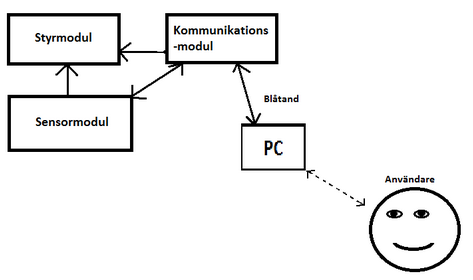
\includegraphics{systemskiss}
\\
Figur 1. \textit{Denna bild visar en översikt av systemet.}

\subsection{Grov beskrivning av produkten}
Roboten kommer att köras på hjul, kunna känna av vad som finns framför, vid sidan av och bakom sin position, greppa tag i medicin eller annan produkt som roboten är avsedd till att leverera, kartlägga ett okänt område och utifrån kartan beräkna samt köra den kortaste vägen från start- till slutdestination. 

\subsection{Produktkomponenter}
Roboten kommer bestå av ett flertalet olika sensorer med avståndsmätning. Minst tre stycken mikroprocessoerer (en per delmodul). 

\subsection{Beroenden till andra system}
Banan som roboten ska köra i måste uppfylla tävlingsreglerna (se bifogat dokument Tävlingsregler.pdf)

\subsection{Ingående delsystem}
Roboten består av tre stycken delsystem (moduler). Kommunikationsmodul, styrmodul och sensormodul. Den förstnämnda sköter kommunikationen mellan roboten och en PC, denna kommunikation sköts via blåtand. Styrmodulen hanterar styrlogik och motorer. Sensormodulen skickar data till kommunikationsmodulen och styrmodulen som tar in dessa och korrigerar riktning efter datan.

\subsection{Avgränsningar}
Miljön som roboten körs i är begränsad på så sätt att den max ska vara 6x6m och passager måste vara bredare än 40 cm. Inga blockerande hinder får förekomma i vägen för roboten, den kan endast röra sig på släta ytor.

\subsection{Designfilosofi}
Målet är att roboten ska vara så snabb och energieffektiv som möjligt och samtidigt utföra uppgiften utan komplikationer. 

\pagebreak

\subsection{Generella krav på hela systemet}
Nedan listas generella krav på hela systemet
\\
\begin{center}
\begin{longtable}{|l|l|p{.70\linewidth}|l|} \hline

Krav nr 1 & 
Original & 
Roboten ska kunna navigera autonomt i en labyrint enl. regler för banan. & 
1 \\ \hline

Krav nr 2 & 
Original & 
Roboten ska reagera på kommandon: fram, fram vänster, fram höger, back, stopp, rotera vänster, rotera höger och kalibrering. & 
1 \\ \hline

Krav nr 3 &
Original &
Kommandon ska ges via en PC via blåtand. &
1 \\ \hline

Krav nr 4 &
Original &
Roboten ska vara utrustad med en gripklo fram, vilken ska kunna plocka upp “förnödenheter” och lämna de på målrutan. &
1 \\ \hline

Krav nr 5 &
Original &
Roboten ska vara moduluppbyggd. &
1 \\ \hline

Krav nr 6 &
Original &
Modulerna skall vara utbytbara. &
1 \\ \hline

Krav nr 7 &
Original &
Varje modul ska innehålla minst en egen processor. &
1 \\ \hline

Krav nr 8 &
Original &
Roboten ska kunna skicka mätdata (avstånd till väggar, avlagd sträcka, vridning), styrbeslut och styrdata till PC via blåtand. &
1 \\ \hline

Krav nr 9 &
Original &
Det ska finnas en brytare på roboten för att växla mellan autonomt läge och fjärrstyrningsläge. &
1 \\ \hline

Krav nr 10 &
Original & 
Projektet skall bedrivas enligt LIPS-modellen.&
1 \\ \hline

Krav nr 11 &
Original &
Vid slutleverans skall en fungerande robot finnas. &
1 \\ \hline

Krav nr 12 &
Original &
Markeringen av målrutan ska göras med en svart ruta på golvet (alternativt med en RFID-tag). &
1 \\ \hline

Krav nr 13 & 
Original & 
Teknisk dokumentation med användaranvisning skall finnas. &
1 \\ \hline

Krav nr 14 &
Original &
Utföra kontinuerlig (veckovis) tidrapportering till beställaren. &
1 \\ \hline

Krav nr 15 &
Original &
Projektet får ta maximalt 1380 arbetstimmar att slutföra. &
1 \\ \hline

Krav nr 16 &
Original &
Tidsplan över hela projektet skall finnas. &
1 \\ \hline

Krav nr 17 &
Original &
En knapp skall finnas som startar roboten i autonomt läge vid tävlingstillfället. &
1 \\ \hline

Krav nr 18 &
Original &
Någon form av styralgoritm skall finnas. &
1 \\ \hline

Krav nr 19 &
Original &
Roboten ska skicka mätdata kontinuerligt till en PC via blåtandslänk. &
1 \\ \hline

Krav nr 20 &
Original &
Roboten ska kunna bestämma den kortaste vägen till målrutan. &
1 \\ \hline

Krav nr 21 &
Original &
Styrmodul skall finnas. &
1 \\ \hline

Krav nr 22 &
Original &
Sensormodul skall finnas. &
1 \\ \hline

Krav nr 23 &
Original &
Kommunikationsmodul skall finnas. &
1 \\ \hline

Krav nr 24 &
Original &
Tävlingsbanan är i enlighet med bifogade regler. &
1 \\ \hline

Krav nr 25 &
Original &
Roboten skall vara med i tävlingen. &
1 \\ \hline

Krav nr 26 &
Original &
Roboten skall klara av upprepade uppdrag i följd. &
1 \\ \hline

Krav nr 27 &
Original &
En karta över miljön roboten rör sig i skall målas upp i 2D. &
2 \\ \hline

Krav nr 28 &
Original &
En LCD-skärm skall finnas på roboten och visa värden från sensorer kontinuerligt. &
2 \\ \hline

Krav nr 29 &
Original &
Roboten bör kunna skicka positionsdata till PC och presentera en karta över grottan med en projektor. &
2 \\ \hline

Krav nr 30 &
Original &
Roboten skall klara passager bredare större än 40 cm. &
2 \\ \hline

\end{longtable}
\end{center}




\pagebreak

\section{Delsystem 1 - Sensormodul}
Delsystem 1 är sensormodulen som består av minst en mikroprocessor samt de olika typer av sensorer som används för att mäta av robotens omgivning.

\subsection{Inledande beskrivning av delsystem 1}
Sensormodulen samlar in mätdata från sina olika sensorer och skickar denna data till styrmodulen (delsystem 2) där denna behandlas och eventuella åtgärder vidtas.

\pagebreak

\section{Delsystem 2 - Styrmodul}
Styrmodulen ska bestå av minst en mikroprocessor.  Denna samlar information från sensor- och kommunikationsmodulerna, och agerar utefter svaren.

\subsection{Inledande beskrivning av delsystem 2}
Styrmodulen ska styra LCD:n, styrlogiken och motorerna.
LCD:n kommer att visa resultat som sensormodulen har skickat till styrmodulen. Styrlogiken kommer bestämma hur motorerna ska kontrolleras, och motorerna kommer utifrån svar från styrlogiken att drivas på.

\pagebreak

\section{Delsystem 3 - Kommunikationsmodul}

\pagebreak

\section{Prestandakrav}
text
\section{Krav på vidareutveckling}
text
\section{Tillförlitlighet}
text
\section{Ekonomi}
De resurser som finns att tillgå är X timmar fördelat på gruppens 6 medlemmar. 
\section{Krav på säkerhet}
text

\pagebreak
\section{Leveranskrav och delleveranser}
Leveranser skall göras senast på nedan nämnda tider och datum om inte annat är överenskommet mellan beställare och projektgrupp
\begin{center}
\begin{longtable}{l p{.8\linewidth} }

3 febr: & 
kl 16.00: Kravspecifikationen ska vara klar. (BP1) \\

16 feb: & 
kl 16.00: Första versionen av projektplan, tidplan och systemskiss ska vara inlämnade till beställaren. \\

20 feb: & 
kl 16.00: Slutgiltig version av projektplan, tidplan och systemskiss ska vara inlämnade till beställaren. \\

5 mars: &
kl 16.00: första version av förstudien (minst 5 sidor) ska skickas till respektive handledare och till er beställare. \\

11 mars: & 
kl 16.00: Första versionen av designspecifikationen ska vara inlämnad till handledaren. \\

24 mars: &
Designspecifikationen ska vara godkänd av handledaren vid ett beslutsmöte BP3. \\

1 april: &
kl 16:00 Version 1.0 av förstudien ska skickas till respektive handledare och till beställare. \\

17 april: & 
Nuvarande design ska vara presenterad för och godkänd av handledaren vid ett beslutsmöte BP4. \\

25 maj: &
Verifiering av kraven (BP5) bör ske i god tid innan redovisningen. Utan detta beslut får ni inte leverera! \\

21 maj: &
Kappan, version 1.0, (exklusive appendix) ska levereras. Se nedan. \\

27 maj: &
Teknisk dokumentation och användarhandledning (båda version 1.0) ska vara inlämnade. Slutversion av skrivarbete skall också skickas med vid detta tillfälle. \\

Vecka 23: &
Redovisning och demonstration.\\

2 juni: &
(preliminärt) 8.15-17 muntliga presentationer och opposition. Tider se nedan. \\

3 juni: &
(preliminärt) 9.15-17 tävlingar utanför café Java. \\

5 juni: &
Efterstudien ska vara inlämnad. Vid denna tidpunkt ska även källkod skickas in i en zip-fil. \\

12 Juni: &
Bärbar dator och övrig utrustning ska vara återlämnade.
\end{longtable}
\end{center}
En tidrapport ska lämnas senast kl 16.00 vid följande datum: 4 febr, 23 febr, 9 mars, 23 mars, 30 mars, 13 april, 20 april, 27 april, 4 maj, 11 maj, 18 maj, 25 maj, 1 juni och 8 juni.

\section{Dokumentation}

\begin{center}
\begin{longtable}{|p{.24\linewidth}|p{.08\linewidth}|p{.25\linewidth}|p{.19\linewidth}|p{.1\linewidth}|}\hline
\textbf{Dokument} & \textbf{Språk} & \textbf{Syfte} & \textbf{Målgrupp} & \textbf{Format} \\ \hline

Kravspecifikation & SE & Listar alla krav som slutprodukten ska uppfylla. & Projektgrupp och beställare & .pdf \\ \hline
Projektplan & SE & Beskriver hur projektet ska utföras & Projektgrupp & .pdf \\ \hline
Tidplan & SE & Beskriver när aktiviteter ska utföras och av vem & Projektgrupp & .xls \\ \hline
Systemskiss & SE & Beskriver hur produkten ska konstrueras& Projektgrupp och beställare & .pdf \\ \hline
Förstudie & SE & Analysera huruvida projektet kan drivas framåt eller inte & Projektgrupp & .pdf \\ \hline
Design-specifikation & SE & Beskriver mer detaljerat hur produkten ska konstrueras & Projektgrupp & .pdf \\ \hline
Kappa & SE & Sammanfattar alla dokument som beställaren kan vara intresserad av & Beställare & .pdf \\ \hline
Teknisk dokumentation & SE & Beskriver hur produkten fungerar & Beställare & .pdf \\ \hline
Användar-handledning & SE & Beskriver hur man använder produkten& Beställare & .pdf \\ \hline
Efterstudie & SE & En reflektion kring hur projektet bedrevs. Vad kunde man ha gjort bättre, etc.& Projektgrupp & .pdf \\ \hline

\end {longtable}
\end {center}

\section{Utbildning}
Vid slutfört projekt skall en utförlig teknisk dokumentation av hela systemet samt alla ingående delsystem finnas. Det skall också finnas en godkänd användarhandledning att tillgå vid projektets slutleverans som ska garantera kunden tillräcklig kunskap för användande av roboten.


\section{Kvalitetskrav}



\section{Underhållsbarhet}
text

\setcounter{secnumdepth}{0}
\section{Referenser}
text
\setcounter{secnumdepth}{2}

\pagebreak

\section{Appendix A}
text



\end{flushleft}




\end{document}

\begin{comment}




\end{comment}